
%%--------------------------------------------------
%% Halliday: Fundamentals of Physics
%%--------------------------------------------------


%% Chapter 07: Kinetic Energy and Work
%%--------------------------------------------------


%% Learning Objectives
%%--------------------------------------------------

%% 7.01: Apply the relationship between a particle's kinetic energy, mass, and speed.
%% 7.02: Identify that kinetic energy is a scalar quantity.


%% Halliday Multiple Choice Questions
%%--------------------------------------------------
\element{halliday-mc}{
\begin{question}{halliday-ch07-q01}
    Which of the following is \emph{not} a correct unit for work?
    \begin{choices}
        \wrongchoice{erg (erg)}
        \wrongchoice{foot pound (\si{\foot\pound})}
      \correctchoice{watt (\si{\watt})}
        \wrongchoice{newton meter (\si{\newton\meter})}
        \wrongchoice{joule (\si{\joule})}
    \end{choices}
\end{question}
}

\element{halliday-mc}{
\begin{question}{halliday-ch07-q02}
    Which of the following groups does \emph{not} contain a scalar quantity?
    \begin{choices}
        \wrongchoice{velocity, force, power}
      \correctchoice{displacement, acceleration, force}
        \wrongchoice{acceleration, speed, work}
        \wrongchoice{energy, work, distance}
        \wrongchoice{pressure, weight, time}
    \end{choices}
\end{question}
}

\element{halliday-mc}{
\begin{question}{halliday-ch07-q03}
    A boy holds a \SI{40}{\newton} weight at arm's length for \SI{10}{\second}.
    His arm is \SI{1.5}{\meter} above the ground. 
    The work done by the force of the boy on the weight while he is holding it is:
    \begin{multicols}{3}
    \begin{choices}
      \correctchoice{zero}
        \wrongchoice{\SI{6.1}{\joule}}
        \wrongchoice{\SI{40}{\joule}}
        \wrongchoice{\SI{60}{\joule}}
        \wrongchoice{\SI{90}{\joule}}
    \end{choices}
    \end{multicols}
\end{question}
}

\element{halliday-mc}{
\begin{question}{halliday-ch07-q04}
    A crate moves \SI{10}{\meter} to the right on a horizontal surface as a woman pulls on it with a 10-N force.
    Rank the situations shown below according to the work done by her force,
        least to greatest.
    \begin{center}
    \begin{tikzpicture}
        %% Ground
        \node[anchor=north,fill,pattern=north east lines,minimum width=2cm, minimum height=0.05cm] at (0,0) {};
        \draw (-1,0) -- (1,0);
        \node[anchor=north,yshift=-0.20cm] at (0,0) {$1$};
        %% Mass
        \node[draw,fill=white!90!black,minimum size=0.75cm,anchor=south] (M) at (0,0) {};
        %% Vectors
        \draw[thick,->] (M.east) -- ++(0:1.5cm) node[anchor=south,pos=0.5] {\SI{10}{\newton}};
    \end{tikzpicture}
    %% NOTE: I technically changed number 2
    %% NOTE: orig is -45, mine is 45
    \begin{tikzpicture}
        %% Ground
        \node[anchor=north,fill,pattern=north east lines,minimum width=2cm, minimum height=0.05cm] at (0,0) {};
        \draw (-1,0) -- (1,0);
        \node[anchor=north,yshift=-0.20cm] at (0,0) {$2$};
        %% Mass
        \node[draw,fill=white!90!black,minimum size=0.75cm,anchor=south] (M) at (0,0) {};
        %% Vectors
        \draw[thick,->] (M.east) -- ++(45:1.5cm) node[anchor=south east,pos=0.8] {\SI{10}{\newton}};
    \end{tikzpicture}
    \begin{tikzpicture}
        %% Ground
        \node[anchor=north,fill,pattern=north east lines,minimum width=2cm, minimum height=0.05cm] at (0,0) {};
        \draw (-1,0) -- (1,0);
        \node[anchor=north,yshift=-0.20cm] at (0,0) {$3$};
        %% Mass
        \node[draw,fill=white!90!black,minimum size=0.75cm,anchor=south] (M) at (0,0) {};
        %% Vectors
        \draw[thick,->] (M.north) -- ++(90:1.5cm) node[anchor=west,pos=0.5] {\SI{10}{\newton}};
    \end{tikzpicture}
    \end{center}
    \begin{multicols}{2}
    \begin{choices}
        \wrongchoice{1, 2, 3}
        \wrongchoice{2, 1, 3}
        \wrongchoice{2, 3, 1}
        \wrongchoice{1, 3, 2}
      \correctchoice{3, 2, 1}
    \end{choices}
    \end{multicols}
\end{question}
}

\element{halliday-mc}{
\begin{question}{halliday-ch07-q05}
    An object moves in a circle at constant speed. 
    The work done by the centripetal force is zero because:
    \begin{choices}
        \wrongchoice{the displacement for each revolution is zero}
        \wrongchoice{the average force for each revolution is zero}
        \wrongchoice{there is no friction}
        \wrongchoice{the magnitude of the acceleration is zero}
      \correctchoice{the centripetal force is perpendicular to the velocity}
    \end{choices}
\end{question}
}

\element{halliday-mc}{
\begin{question}{halliday-ch07-q06}
    An object of mass \SI{1}{\gram} is whirled in a horizontal circle of radius \SI{0.5}{\meter} at a constant speed of \SI{2}{\meter\per\second}. 
    The work done on the object during one revolution is:
    \begin{multicols}{3}
    \begin{choices}
      \correctchoice{zero}
        \wrongchoice{\SI{1}{\joule}}
        \wrongchoice{\SI{2}{\joule}}
        \wrongchoice{\SI{4}{\joule}}
        \wrongchoice{\SI{16}{\joule}}
    \end{choices}
    \end{multicols}
\end{question}
}

\element{halliday-mc}{
\begin{question}{halliday-ch07-q07}
    The work done by gravity during the descent of a projectile:
    \begin{choices}
      \correctchoice{is positive}
        \wrongchoice{is negative}
        \wrongchoice{is zero}
        \wrongchoice{depends for its sign on the direction of the $y$ axis}
        \wrongchoice{depends for its sign on the direction of both the $x$ and $y$ axes}
    \end{choices}
\end{question}
}

\element{halliday-mc}{
\begin{question}{halliday-ch07-q08}
    A baseball is hit high into the upper bleachers of left field. 
    Over its entire flight the work done by gravity and the work done by air resistance,
        respectively, are:
    \begin{choices}
        \wrongchoice{positive; positive}
        \wrongchoice{positive; negative}
        \wrongchoice{negative; positive}
      \correctchoice{negative; negative}
        \wrongchoice{unknown since vital information is lacking}
    \end{choices}
\end{question}
}

\element{halliday-mc}{
\begin{question}{halliday-ch07-q09}
    A line drive to the shortstop is caught at the same height as it was originally hit. 
    Over its entire flight the work done by gravity and the work done by air resistance, respectively, are:
    \begin{choices}
        \wrongchoice{zero; positive}
      \correctchoice{zero; negative}
        \wrongchoice{positive; negative}
        \wrongchoice{negative; positive}
        \wrongchoice{negative; negative}
    \end{choices}
\end{question}
}

\element{halliday-mc}{
\begin{question}{halliday-ch07-q10}
    A \SI{2}{\kilo\gram} object is moving at \SI{3}{\meter\per\second}.
    A \SI{4}{\newton} force is applied in the direction of motion and then removed after the object has traveled an additional \SI{5}{\meter}. 
    The work done by this force is:
    \begin{multicols}{3}
    \begin{choices}
        \wrongchoice{\SI{12}{\joule}}
        \wrongchoice{\SI{15}{\joule}}
        \wrongchoice{\SI{18}{\joule}}
      \correctchoice{\SI{20}{\joule}}
        \wrongchoice{\SI{38}{\joule}}
    \end{choices}
    \end{multicols}
\end{question}
}

\element{halliday-mc}{
\begin{question}{halliday-ch07-q11}
    A sledge (including load) weighs \SI{5000}{\newton}. 
    It is pulled on level snow by a dog team exerting a horizontal force on it. 
    The coefficient of kinetic friction between sledge and snow is \num{0.05}. 
    How much work is done by the dog team pulling the sledge \SI{1000}{\meter} at constant speed?
    \begin{multicols}{2}
    \begin{choices}
        \wrongchoice{\SI{2.5e4}{\joule}}
      \correctchoice{\SI{2.5e5}{\joule}}
        \wrongchoice{\SI{5.0e5}{\joule}}
        \wrongchoice{\SI{2.5e6}{\joule}}
        \wrongchoice{\SI{5.0e6}{\joule}}
    \end{choices}
    \end{multicols}
\end{question}
}

\element{halliday-mc}{
\begin{question}{halliday-ch07-q12}
    Camping equipment weighing \SI{6000}{\newton} is pulled across a frozen lake by means of a horizontal rope. 
    The coefficient of kinetic friction is \num{0.05}. 
    The work done by the campers in pulling the equipment \SI{1000}{\meter} at constant velocity is:
    \begin{multicols}{2}
    \begin{choices}
        \wrongchoice{\SI{3.1e4}{\joule}}
        \wrongchoice{\SI{1.5e5}{\joule}}
      \correctchoice{\SI{3.0e5}{\joule}}
        \wrongchoice{\SI{2.9e6}{\joule}}
        \wrongchoice{\SI{6.0e6}{\joule}}
    \end{choices}
    \end{multicols}
\end{question}
}

\element{halliday-mc}{
\begin{question}{halliday-ch07-q13}
    Camping equipment weighing \SI{6000}{\newton} is pulled across a frozen lake by means of a horizontal rope. 
    The coefficient of kinetic friction is \num{0.05}. 
    How much work is done by the campers in pulling the equipment \SI{1000}{\meter} if its speed is increasing at the constant rate of \SI{0.20}{\meter\per\second\squared}?
    \begin{multicols}{2}
    \begin{choices}
        \wrongchoice{\SI{-1.2e6}{\joule}}
        \wrongchoice{\SI{1.8e5}{\joule}}
        \wrongchoice{\SI{3.0e5}{\joule}}
      \correctchoice{\SI{4.2e5}{\joule}}
        \wrongchoice{\SI{1.2e6}{\joule}}
    \end{choices}
    \end{multicols}
\end{question}
}

\element{halliday-mc}{
\begin{question}{halliday-ch07-q14}
    A \SI{1}{\kilo\gram} block is lifted vertically \SI{1}{\meter} by a boy. 
    The work done by the boy is about:
    \begin{multicols}{3}
    \begin{choices}
        \wrongchoice{\SI{1}{\foot\pound}}
        \wrongchoice{\SI{1}{\joule}}
      \correctchoice{\SI{10}{\joule}}
        \wrongchoice{\SI{0.1}{\joule}}
        \wrongchoice{zero}
    \end{choices}
    \end{multicols}
\end{question}
}

\element{halliday-mc}{
\begin{question}{halliday-ch07-q15}
    A \SI{0.50}{\kilo\gram} object moves in a horizontal circular track with a radius of \SI{2.5}{\meter}. 
    An external force of \SI{3.0}{\newton},
        always tangent to the track, causes the object to speed up as it goes around. 
    The work done by the external force as the mass makes one revolution is:
    \begin{multicols}{3}
    \begin{choices}
        \wrongchoice{\SI{24}{\joule}}
      \correctchoice{\SI{47}{\joule}}
        \wrongchoice{\SI{59}{\joule}}
        \wrongchoice{\SI{94}{\joule}}
        \wrongchoice{\SI{120}{\joule}}
    \end{choices}
    \end{multicols}
\end{question}
}

\element{halliday-mc}{
\begin{question}{halliday-ch07-q16}
    A man pulls a \SI{100}{\newton} crate up a frictionless \ang{30} slope \SI{5}{\meter} high, as shown. 
    \begin{center}
    \begin{tikzpicture}[scale=0.9]
        %% Surface
        \node[anchor=north,fill,pattern=north east lines,minimum width=6cm, minimum height=0.05cm] at (2,0) {};
        \draw (-1,0) -- (5,0);
        %% Include plane, triangle
        \draw[thick] (0,0) -- (30:5cm) -- ++(270:2.5cm) node[pos=0.5,anchor=east] {\SI{5}{\meter}};
        \draw[<->] (0:1) arc (0:30:1) node[pos=0.5,anchor=west] {\ang{30}};
        %% Masses
        \node[draw,fill=white!90!black,rectangle,minimum size=1.4cm,rotate=30,anchor=south] (M) at (30:2) {\SI{100}{\newton}};
        %% Rope
        \draw[very thick,->] (M.south east) ++(120:0.5) -- (4.95,3.43) arc (120:20:0.5) -- ++ (-70:2) node[anchor=north,text width=4em,text centered] {pull from man};
        %% Pulley
        \draw[fill=white!90!black] (30:6cm) circle (0.50cm);
        \draw (30:5cm) -- ++ (30:1cm);
        \draw[fill] (30:6cm) circle (1.5pt);
    \end{tikzpicture}
    \end{center}
    Assuming that the crate moves at constant speed,
        the work done by the man is:
    \begin{multicols}{3}
    \begin{choices}
        \wrongchoice{\SI{-500}{\joule}}
        \wrongchoice{\SI{-250}{\joule}}
        \wrongchoice{zero}
        \wrongchoice{\SI{250}{\joule}}
      \correctchoice{\SI{500}{\joule}}
        %% Added for symmetry
        \wrongchoice{\SI{433}{\joule}}
    \end{choices}
    \end{multicols}
\end{question}
}

\element{halliday-mc}{
\begin{question}{halliday-ch07-q17}
    A man pushes an \SI{80}{\newton} crate a distance of \SI{5.0}{\meter} upward along a frictionless slope that makes an angle of \ang{30} with the horizontal.
    His force is parallel to the slope. 
    If the speed of the crate decreases at a rate of \SI{1.5}{\meter\per\second\squared},
        then the work done by the man is:
    \begin{multicols}{3}
    \begin{choices}
        \wrongchoice{\SI{-200}{\joule}}
        \wrongchoice{\SI{61}{\joule}}
      \correctchoice{\SI{140}{\joule}}
        \wrongchoice{\SI{200}{\joule}}
        \wrongchoice{\SI{260}{\joule}}
    \end{choices}
    \end{multicols}
\end{question}
}

\element{halliday-mc}{
\begin{question}{halliday-ch07-q18}
    A man pushes an \SI{80}{\newton} crate a distance of \SI{5.0}{\meter} upward along a frictionless slope that makes an angle of \ang{30} with the horizontal. 
    The force he exerts is parallel to the slope. 
    If the speed of the crate is constant,
        then the work done by the man is:
    \begin{multicols}{3}
    \begin{choices}
        \wrongchoice{\SI{-200}{\joule}}
        \wrongchoice{\SI{61}{\joule}}
        \wrongchoice{\SI{140}{\joule}}
      \correctchoice{\SI{200}{\joule}}
        \wrongchoice{\SI{260}{\joule}}
    \end{choices}
    \end{multicols}
\end{question}
}

\element{halliday-mc}{
\begin{question}{halliday-ch07-q19}
    An \SI{80}{\newton} crate slides with constant speed a distance of \SI{5.0}{\meter} downward along a rough slope that makes an angle of \ang{30} with the horizontal. 
    The work done by the force of gravity is:
    \begin{multicols}{3}
    \begin{choices}
        \wrongchoice{\SI{-400}{\joule}}
        \wrongchoice{\SI{-200}{\joule}}
        \wrongchoice{\SI{-69}{\joule}}
      \correctchoice{\SI{200}{\joule}}
        \wrongchoice{\SI{400}{\joule}}
    \end{choices}
    \end{multicols}
\end{question}
}

\element{halliday-mc}{
\begin{question}{halliday-ch07-q20}
    A man pulls a sled along a rough horizontal surface by applying a constant force $F$ at an angle $\theta$ above the horizontal. 
    In pulling the sled a horizontal distance $d$,
        the work done by the man is:
    \begin{multicols}{3}
    \begin{choices}
        \wrongchoice{$F d$}
      \correctchoice{$F d \cos\theta$}
        \wrongchoice{$F d \sin\theta$}
        \wrongchoice{$\dfrac{F d}{\cos\theta}$}
        \wrongchoice{$\dfrac{F d}{\sin\theta}$}
    \end{choices}
    \end{multicols}
\end{question}
}

%\element{halliday-mc}{
%\begin{question}{halliday-ch07-q21}
%    A man wishes to pull a crate \SI{15}{\meter} across a rough floor by exerting a force of \SI{100}{\newton}.
%    The coefficient of kinetic friction is \num{0.25}. 
%    %For the least amount of work to be performed on the crate,
%    For the man to do the least work,
%        the angle between the force and the horizontal should be:
%    \begin{multicols}{3}
%    \begin{choices}
%        %% NOTE: very tricky
%        %% NOTE: it is necessary to assume a large mass
%      \correctchoice{\ang{0}}
%        \wrongchoice{\ang{14}}
%        \wrongchoice{\ang{43}}
%        \wrongchoice{\ang{66}}
%        \wrongchoice{\ang{76}}
%    \end{choices}
%    \end{multicols}
%\end{question}
%}

\element{halliday-mc}{
\begin{question}{halliday-ch07-q22}
    A particle moves \SI{5}{\meter} in the positive x direction while being acted upon by a constant force
        ${F = \left(\SI{4}{\newton}\right)\hat{\imath} + \left(\SI{2}{\newton}\right)\hat{\jmath} - \left(\SI{4}{\newton}\right)\hat{k}}$.
    The work done on the particle by this force is:
    \begin{multicols}{2}
    \begin{choices}
      \correctchoice{\SI{20}{\joule}}
        \wrongchoice{\SI{10}{\joule}}
        \wrongchoice{\SI{-20}{\joule}}
        \wrongchoice{\SI{30}{\joule}}
        \wrongchoice{is impossible to calculate without knowing other forces}
    \end{choices}
    \end{multicols}
\end{question}
}

\element{halliday-mc}{
\begin{question}{halliday-ch07-q23}
    A block is attached to the end of an ideal spring and moved from coordinate $x_i$ to coordinate $x_f$.
    The relaxed position is at $x=0$. 
    The work done by spring is positive if:
    \begin{choices}
        \wrongchoice{$x_i=\SI{2}{\centi\meter}$ and  $x_f=\SI{4}{\centi\meter}$}
        \wrongchoice{$x_i=\SI{-2}{\centi\meter}$ and $x_f=\SI{4}{\centi\meter}$}
        \wrongchoice{$x_i=\SI{-2}{\centi\meter}$ and $x_f=\SI{-4}{\centi\meter}$}
        \wrongchoice{$x_i=\SI{2}{\centi\meter}$ and  $x_f=\SI{-4}{\centi\meter}$}
      \correctchoice{$x_i=\SI{-4}{\centi\meter}$ and $x_f=\SI{-2}{\centi\meter}$}
    \end{choices}
\end{question}
}

%\element{halliday-mc}{
%\begin{question}{halliday-ch07-q24}
%    An ideal spring, with a pointer attached to its end, hangs next to a scale. 
%    With a \SI{100}{\newton} weight attached,
%        the pointer indicates ``40'' on the scale as shown. 
%    \begin{center}
%    \begin{tikzpicture}
%        %% NOTE: jphafner
%        %% Ceiling
%        \node[anchor=south,fill,pattern=north east lines,minimum width=4cm, minimum height=0.05cm] at (0,0) {};
%        \draw (-2,0) -- (2,0);
%        %% Masses
%        \node[draw,fill=white!90!black,rectangle,anchor=north,minimum size=1.4cm] (M) at (0,-2.5) {\SI{100}{\newton}};
%        %% Springs
%        \draw[thick,decoration={aspect=0.2,segment length=2.0mm,amplitude=3mm,coil},decorate] (0,0) -- (0,-2);
%        \draw[thick] (0,-2) -- (M.north);
%        %% Ruler
%        \draw[thick,->] (0,-2) -- ++(0:1cm);
%        %\begin{scope}[shift={ }]
%        %    \draw (0,0) rectangle (0.5,2);
%        %    \foreach \y in { } {
%        %        \draw (0,\y) -- (1em,\y);
%        %    }
%        %\end{scope}
%    \end{tikzpicture}
%    \end{center}
%    Using a \SI{200}{\newton} weight instead results in ``60'' on the scale. 
%    Using an unknown weight $X$ instead results in ``30'' on the scale. 
%    The weight of $X$ is:
%    \begin{multicols}{3}
%    \begin{choices}
%        \wrongchoice{\SI{10}{\newton}}
%        \wrongchoice{\SI{20}{\newton}}
%        \wrongchoice{\SI{30}{\newton}}
%        \wrongchoice{\SI{40}{\newton}}
%      \correctchoice{\SI{50}{\newton}}
%    \end{choices}
%    \end{multicols}
%\end{question}
%}

%% NOTE: alternate question comparing the work performed on x and Z+Y
%\element{halliday-mc}{
%\begin{question}{halliday-ch07-q25}
%    Three identical ideal springs ($X$, $Y$, $Z$) are arranged as shown. 
%    \begin{center}
%    \begin{tikzpicture}
%        %% NOTE:
%    \end{tikzpicture}
%    \end{center}
%    When a \SI{4.0}{\kilo\gram} mass is hung on $X$,
%    the mass descends \SI{3.0}{\centi\meter}.
%    When a \SI{6.0}{\kilo\gram} mass is hung on $Y$,
%        the mass descends:
%    \begin{multicols}{3}
%    \begin{choices}
%        \wrongchoice{\SI{2.0}{\centi\meter}}
%        \wrongchoice{\SI{4.0}{\centi\meter}}
%        \wrongchoice{\SI{4.5}{\centi\meter}}
%        \wrongchoice{\SI{6.0}{\centi\meter}}
%      \correctchoice{\SI{9.0}{\centi\meter}}
%    \end{choices}
%    \end{multicols}
%\end{question}
%}

\element{halliday-mc}{
\begin{question}{halliday-ch07-q26}
    When a certain rubber band is stretched a distance $x$,
        it exerts a restoring force of magnitude $F = Ax$, where $A$ is a constant. 
    The work done by a person in stretching this rubber band from $x=0$ to $x=L$,
        beginning and ending at rest, is:
    \begin{multicols}{3}
    \begin{choices}
        \wrongchoice{$AL^2$}
        \wrongchoice{$A + 2L$}
        \wrongchoice{$A + 2L^2$}
        \wrongchoice{$\dfrac{A}{L}$}
      \correctchoice{$\dfrac{AL^2}{2}$}
    \end{choices}
    \end{multicols}
\end{question}
}

\element{halliday-mc}{
\begin{question}{halliday-ch07-q27}
    When a certain rubber band is stretched a distance $x$,
        it exerts a restoring force of magnitude $F=ax+bx^2$,
        where $a$ and $b$ are constants. 
    The work done in stretching this rubber band from $x=0$ to $x=L$ is:
    \begin{multicols}{2}
    \begin{choices}
        \wrongchoice{$aL^2 + bLx^3$}
        \wrongchoice{$aL + 2bL^2$}
        \wrongchoice{$a + 2bL$}
        \wrongchoice{$bL$}
      \correctchoice{$\dfrac{aL^2}{2} + \dfrac{bL^3}{3}$}
    \end{choices}
    \end{multicols}
\end{question}
}

\element{halliday-mc}{
\begin{question}{halliday-ch07-q28}
    An ideal spring is hung vertically from the ceiling. 
    When a \SI{2.0}{\kilo\gram} mass hangs at rest from it the spring is extended \SI{6.0}{\centi\meter} from its relaxed length. 
    A downward external force is now applied to the mass to extend the spring an additional \SI{10}{\centi\meter}.
    While the spring is being extended by the force,
        the work done by the spring is:
    \begin{multicols}{2}
    \begin{choices}
      \correctchoice{\SI{-3.6}{\joule}}
        \wrongchoice{\SI{-3.3}{\joule}}
        \wrongchoice{\SI{-3.4e-5}{\joule}}
        \wrongchoice{\SI{3.3}{\joule}}
        \wrongchoice{\SI{3.6}{\joule}}
    \end{choices}
    \end{multicols}
\end{question}
}

\element{halliday-mc}{
\begin{question}{halliday-ch07-q29}
    An ideal spring is hung vertically from the ceiling. 
    When a \SI{2.0}{\kilo\gram} block hangs at rest from it the spring is extended \SI{6.0}{\centi\meter} from its relaxed length. 
    A upward external force is then applied to the block to move it upward a distance of \SI{16}{\centi\meter}.
    While the block is moving upward the work done by the spring is:
    \begin{multicols}{3}
    \begin{choices}
      \correctchoice{\SI{-1.0}{\joule}}
        \wrongchoice{\SI{-0.52}{\joule}}
        \wrongchoice{\SI{-0.26}{\joule}}
        \wrongchoice{\SI{0.52}{\joule}}
        \wrongchoice{\SI{1.0}{\joule}}
    \end{choices}
    \end{multicols}
\end{question}
}

\element{halliday-mc}{
\begin{question}{halliday-ch07-q30}
    Which of the following bodies has the largest kinetic energy?
    \begin{choices}
        \wrongchoice{Mass $3M$ and speed $V$}
        \wrongchoice{Mass $3M$ and speed $2V$}
      \correctchoice{Mass $2M$ and speed $3V$}
        \wrongchoice{Mass $M$ and speed $4V$}
        \wrongchoice{All have the same kinetic energy}
    \end{choices}
\end{question}
}

\element{halliday-mc}{
\begin{question}{halliday-ch07-q31}
    Two trailers, $X$ with mass \SI{500}{\kilo\gram} and $Y$ with mass \SI{2000}{\kilo\gram},
        are being pulled at the same speed.
    The ratio of the kinetic energy of $Y$ to that of $X$ is:
    \begin{multicols}{3}
    \begin{choices}
        \wrongchoice{$1:1$}
        \wrongchoice{$2:1$}
      \correctchoice{$4:1$}
        \wrongchoice{$9:1$}
        \wrongchoice{$1500:1$}
    \end{choices}
    \end{multicols}
\end{question}
}

\element{halliday-mc}{
\begin{question}{halliday-ch07-q32}
    A \SI{8000}{\newton} car is traveling at \SI{12}{\meter\per\second} along a horizontal road when the brakes are applied. 
    The car skids to a stop in \SI{4.0}{\second}.
    How much kinetic energy does the car lose in this time?
    \begin{multicols}{2}
    \begin{choices}
        \wrongchoice{\SI{4.8e4}{\joule}}
      \correctchoice{\SI{5.9e4}{\joule}}
        \wrongchoice{\SI{1.2e5}{\joule}}
        \wrongchoice{\SI{5.8e5}{\joule}}
        \wrongchoice{\SI{4.8e6}{\joule}}
    \end{choices}
    \end{multicols}
\end{question}
}

\element{halliday-mc}{
\begin{question}{halliday-ch07-q33}
    The velocity of a particle moving along the $x$ axis changes from $v_i$ to $v_f$.
    For which values of $v_i$ and $v_f$ is the total work done on the particle positive?
    \begin{choices}
        \wrongchoice{$v_i=\SI{5}{\meter\per\second}$,  $v_f=\SI{2}{\meter\per\second}$}
        \wrongchoice{$v_i=\SI{5}{\meter\per\second}$,  $v_f=\SI{-2}{\meter\per\second}$}
        \wrongchoice{$v_i=\SI{-5}{\meter\per\second}$, $v_f=\SI{-2}{\meter\per\second}$}
        \wrongchoice{$v_i=\SI{-5}{\meter\per\second}$, $v_f=\SI{2}{\meter\per\second}$}
      \correctchoice{$v_i=\SI{2}{\meter\per\second}$,  $v_f=\SI{-5}{\meter\per\second}$}
    \end{choices}
\end{question}
}

\element{halliday-mc}{
\begin{question}{halliday-ch07-q34}
    An object is constrained by a cord to move in a circular path of radius \SI{0.5}{\meter} on a horizontal frictionless surface. 
    The cord will break if its tension exceeds \SI{16}{\newton}. 
    The maximum kinetic energy the object can have is:
    \begin{multicols}{3}
    \begin{choices}
      \correctchoice{\SI{4}{\joule}}
        \wrongchoice{\SI{8}{\joule}}
        \wrongchoice{\SI{16}{\joule}}
        \wrongchoice{\SI{32}{\joule}}
        \wrongchoice{\SI{64}{\joule}}
    \end{choices}
    \end{multicols}
\end{question}
}

\element{halliday-mc}{
\begin{question}{halliday-ch07-q35}
    The weight of an object on the moon is one-sixth of its weight on Earth. 
    The ratio of the kinetic energy of a body on Earth moving with speed $V$ to that of the same body moving with speed $V$ on the moon is:
    \begin{multicols}{3}
    \begin{choices}
        \wrongchoice{$6:1$}
        \wrongchoice{$36:1$}
      \correctchoice{$1:1$}
        \wrongchoice{$1:6$}
        \wrongchoice{$1:36$}
    \end{choices}
    \end{multicols}
\end{question}
}

\element{halliday-mc}{
\begin{question}{halliday-ch07-q36}
    Which of the following is the correct combination of dimensions for energy?
    \begin{multicols}{3}
    \begin{choices}
        \wrongchoice{$MLT$}
        \wrongchoice{$\dfrac{\mathrm{L}\mathrm{T}^2}{\mathrm{M}}$}
      \correctchoice{$\dfrac{\mathrm{M}\mathrm{L}^2}{\mathrm{T}^2}$}
        \wrongchoice{$\dfrac{\mathrm{M}^2\mathrm{L}^3}{\mathrm{T}}$}
        \wrongchoice{$\dfrac{\mathrm{M}\mathrm{L}}{\mathrm{T}^2}$}
    \end{choices}
    \end{multicols}
\end{question}
}

\element{halliday-mc}{
\begin{question}{halliday-ch07-q37}
    The amount of work required to stop a moving object is equal to:
    \begin{choices}
        \wrongchoice{the velocity of the object}
      \correctchoice{the kinetic energy of the object}
        \wrongchoice{the mass of the object times its acceleration}
        \wrongchoice{the mass of the object times its velocity}
        \wrongchoice{the square of the velocity of the object}
    \end{choices}
\end{question}
}

\element{halliday-mc}{
\begin{question}{halliday-ch07-q38}
    A \SI{5.0}{\kilo\gram} cart is moving horizontally at \SI{6.0}{\meter\per\second}.
    In order to change its speed to \SI{10.0}{\meter\per\second},
        the net work done on the cart must be:
    \begin{multicols}{3}
    \begin{choices}
        \wrongchoice{\SI{40}{\joule}}
        \wrongchoice{\SI{90}{\joule}}
      \correctchoice{\SI{160}{\joule}}
        \wrongchoice{\SI{400}{\joule}}
        \wrongchoice{\SI{550}{\joule}}
    \end{choices}
    \end{multicols}
\end{question}
}

\element{halliday-mc}{
\begin{question}{halliday-ch07-q39}
    A crate is initially at rest on a horizontal frictionless table. 
    A constant horizontal force $F$ is applied. 
    %Which of the following five graphs is a correct plot of work $W$ as a function of the crate's speed $v$?
    Which of the following five graphs is a correct plot of work as a function of the crate's speed?
    \begin{multicols}{2}
    \begin{choices}
        \AMCboxDimensions{down=-2.5em}
        \wrongchoice{
            \begin{tikzpicture}
                \begin{axis}[
                    axis y line=left,
                    axis x line=bottom,
                    axis line style={->},
                    xlabel={speed},
                    xtick=\empty,
                    ylabel={work},
                    ytick=\empty,
                    xmin=0,xmax=11,
                    ymin=0,ymax=11,
                    width=0.95\columnwidth,
                    very thin,
                ]
                \addplot[line width=1pt,domain=0:10]{x};
                \end{axis}
            \end{tikzpicture}
        }
        \wrongchoice{
            \begin{tikzpicture}
                \begin{axis}[
                    axis y line=left,
                    axis x line=bottom,
                    axis line style={->},
                    xlabel={speed},
                    xtick=\empty,
                    ylabel={work},
                    ytick=\empty,
                    xmin=0,xmax=11,
                    ymin=0,ymax=11,
                    width=0.95\columnwidth,
                    very thin,
                ]
                \addplot[dashed,domain=0:10] {x};
                \addplot[line width=1pt,domain=0:6]{x};
                \addplot[line width=1pt,domain=6:10]{6+2*(x-6)};
                \end{axis}
            \end{tikzpicture}
        }
        \wrongchoice{
            \begin{tikzpicture}
                \begin{axis}[
                    axis y line=left,
                    axis x line=bottom,
                    axis line style={->},
                    xlabel={speed},
                    xtick=\empty,
                    ylabel={work},
                    ytick=\empty,
                    xmin=0,xmax=11,
                    ymin=0,ymax=11,
                    width=0.95\columnwidth,
                    very thin,
                ]
                \addplot[dashed,domain=0:10] {x};
                \addplot[line width=1pt,domain=0:6]{x};
                \addplot[line width=1pt,domain=6:10]{x - 0.2*(x-6)*(x-6)};
                \end{axis}
            \end{tikzpicture}
        }
        %% ANS is D
        \correctchoice{
            \begin{tikzpicture}
                \begin{axis}[
                    axis y line=left,
                    axis x line=bottom,
                    axis line style={->},
                    xlabel={speed},
                    xtick=\empty,
                    ylabel={work},
                    ytick=\empty,
                    xmin=0,xmax=11,
                    ymin=0,ymax=11,
                    width=0.95\columnwidth,
                    very thin,
                ]
                \addplot[line width=1pt,domain=0:10] {0.1*x*x};
                \end{axis}
            \end{tikzpicture}
        }
        \wrongchoice{
            \begin{tikzpicture}
                \begin{axis}[
                    axis y line=left,
                    axis x line=bottom,
                    axis line style={->},
                    xlabel={speed},
                    xtick=\empty,
                    ylabel={work},
                    ytick=\empty,
                    xmin=0,xmax=11,
                    ymin=0,ymax=11,
                    width=0.95\columnwidth,
                    very thin,
                ]
                %\addplot[line width=1pt,domain=0:10] {10-0.1*(x-10)*(x-10)};
                %% Changed from original
                \addplot[line width=1pt,domain=0:10] {3.1*sqrt(x)};
                \end{axis}
            \end{tikzpicture}
        }
        %% Added for Symmetry
        \wrongchoice{
            \begin{tikzpicture}
                \begin{axis}[
                    axis y line=left,
                    axis x line=bottom,
                    axis line style={->},
                    xlabel={speed},
                    xtick=\empty,
                    ylabel={work},
                    ytick=\empty,
                    xmin=0,xmax=11,
                    ymin=0,ymax=11,
                    width=0.95\columnwidth,
                    very thin,
                ]
                \addplot[line width=1pt,domain=0:10] {10/x};
                \end{axis}
            \end{tikzpicture}
        }
    \end{choices}
    \end{multicols}
\end{question}
}

\element{halliday-mc}{
\begin{question}{halliday-ch07-q40}
    An \SI{8}{\newton} block slides down an incline.
    It has an initial speed of \SI{7}{\meter\per\second}. 
    The work done by the resultant force on this block is:
    \begin{multicols}{2}
    \begin{choices}
        \wrongchoice{\SI{3}{\joule}}
        \wrongchoice{\SI{6}{\joule}}
        \wrongchoice{\SI{56}{\joule}}
      \correctchoice{impossible to calculate without more information}
        \wrongchoice{none of these}
    \end{choices}
    \end{multicols}
\end{question}
}

\element{halliday-mc}{
\begin{question}{halliday-ch07-q41}
    A \SI{4}{\kilo\gram} cart starts up an incline with a speed of \SI{3}{\meter\per\second} and comes to rest \SI{2}{\meter} up the incline.
    The total work done on the car is:
    \begin{multicols}{2}
    \begin{choices}
        \wrongchoice{\SI{6}{\joule}}
        \wrongchoice{\SI{8}{\joule}}
        \wrongchoice{\SI{12}{\joule}}
      \correctchoice{\SI{18}{\joule}}
        \wrongchoice{impossible to calculate without more information}
    \end{choices}
    \end{multicols}
\end{question}
}

\element{halliday-mc}{
\begin{question}{halliday-ch07-q42}
    Two objects with masses of $m_1$ and $m_2$ have the same kinetic energy and are both moving to the right. 
    The same constant force $F$ is applied to the left to both masses. 
    If $m_1 = 4m_2$,
        the ratio of the stopping distance of $m_1$ to that of $m_2$ is:
    \begin{multicols}{3}
    \begin{choices}
        \wrongchoice{$1:4$}
        \wrongchoice{$4:1$}
        \wrongchoice{$1:2$}
        \wrongchoice{$2:1$}
      \correctchoice{$1:1$}
    \end{choices}
    \end{multicols}
\end{question}
}

\element{halliday-mc}{
\begin{question}{halliday-ch07-q43}
    A Boston Red Sox baseball player catches a ball of mass $m$ that is moving toward him with speed $v$. 
    While bringing the ball to rest,
        his hand moves back a distance $d$. 
    Assuming constant deceleration,
        the horizontal force exerted on the ball by his hand is:
    \begin{multicols}{3}
    \begin{choices}
        \wrongchoice{$\dfrac{mv}{d}$}
        \wrongchoice{$mvd$}
        \wrongchoice{$\dfrac{mv^2}{d}$}
        \wrongchoice{$\dfrac{2mv}{d}$}
      \correctchoice{$\dfrac{mv^2}{2d}$}
    \end{choices}
    \end{multicols}
\end{question}
}

\element{halliday-mc}{
\begin{question}{halliday-ch07-q44}
    A \SI{0.50}{\kilo\gram} object moves on a horizontal circular track with a radius of \SI{2.5}{\meter}. 
    An external force of \SI{3.0}{\newton}, always tangent to the track,
        causes the object to speed up as it goes around. 
    If it starts from rest its speed at the end of one revolution is:
    \begin{multicols}{3}
    \begin{choices}
        \wrongchoice{\SI{9.8}{\meter\per\second}}
      \correctchoice{\SI{14}{\meter\per\second}}
        \wrongchoice{\SI{15}{\meter\per\second}}
        \wrongchoice{\SI{19}{\meter\per\second}}
        \wrongchoice{\SI{21}{\meter\per\second}}
    \end{choices}
    \end{multicols}
\end{question}
}

\element{halliday-mc}{
\begin{question}{halliday-ch07-q45}
    A \SI{0.50}{\kilo\gram} object moves on a horizontal frictionless circular track with a radius of \SI{2.5}{\meter}. 
    An external force of \SI{3.0}{\newton}, always tangent to the track,
        causes the object to speed up as it goes around. 
    If it starts from rest,
        then at the end of one revolution the radial component of the force of the track on it is:
    \begin{multicols}{3}
    \begin{choices}
        \wrongchoice{\SI{19}{\newton}}
      \correctchoice{\SI{38}{\newton}}
        \wrongchoice{\SI{47}{\newton}}
        \wrongchoice{\SI{75}{\newton}}
        \wrongchoice{\SI{96}{\newton}}
    \end{choices}
    \end{multicols}
\end{question}
}

\element{halliday-mc}{
\begin{question}{halliday-ch07-q46}
    A \SI{2}{\kilo\gram} block is attached to a horizonal ideal spring with a spring constant of \SI{200}{\newton\per\meter}. 
    When the spring has its equilibrium length the block is given a speed of \SI{5}{\meter\per\second}. 
    What is the maximum elongation of the spring?
    \begin{multicols}{3}
    \begin{choices}
        \wrongchoice{zero}
        \wrongchoice{\SI{0.05}{\meter}}
        % fixed typo
      %\correctchoice{\SI{5}{\meter}}
      \correctchoice{\SI{0.5}{\meter}}
        \wrongchoice{\SI{10}{\meter}}
        \wrongchoice{\SI{100}{\meter}}
    \end{choices}
    \end{multicols}
\end{question}
}

\element{halliday-mc}{
\begin{question}{halliday-ch07-q47}
    At time $t=0$ a particle starts moving along the $x$ axis. 
    If its kinetic energy increases uniformly with $t$ the net force acting on it must be:
    \begin{choices}
        \wrongchoice{constant}
        \wrongchoice{proportional to $t$}
        \wrongchoice{inversely proportional to $t$}
        \wrongchoice{proportional to $\sqrt{t}$}
      \correctchoice{proportional to $\dfrac{1}{\sqrt{t}}$}
    \end{choices}
\end{question}
}

\element{halliday-mc}{
\begin{question}{halliday-ch07-q48}
    At time $t=0$ a \SI{2}{\kilo\gram} particle has a velocity of $\left(\SI{4}{\meter\per\second}\right)\hat{\imath} - \left(\SI{3}{\meter\per\second}\right)\hat{\jmath}$.
    At $t=\SI{3}{\second}$ its velocity is $\left(\SI{2}{\meter\per\second}\right)\hat{\imath} + \left(\SI{3}{\meter\per\second}\right)\hat{\jmath}$.
    During this time the work done on it was:
    \begin{multicols}{2}
    \begin{choices}
        \wrongchoice{\SI{4}{\joule}}
        \wrongchoice{\SI{-4}{\joule}}
      \correctchoice{\SI{-12}{\joule}}
        \wrongchoice{\SI{-40}{\joule}}
        \wrongchoice{$\left(\SI{4}{\joule}\right)\hat{\imath} + \left(\SI{36}{\joule}\right)\hat{\jmath}$}
    \end{choices}
    \end{multicols}
\end{question}
}

\element{halliday-mc}{
\begin{question}{halliday-ch07-q49}
    A particle starts from rest at time $t=0$ and moves along the $x$ axis. 
    If the net force on it is proportional to t,
        its kinetic energy is proportional to:
    \begin{multicols}{2}
    \begin{choices}
        \wrongchoice{$t$}
        \wrongchoice{$t^2$}
      \correctchoice{$t^4$}
        \wrongchoice{$t^{-2}$}
        \wrongchoice{none of the provided}
    \end{choices}
    \end{multicols}
\end{question}
}

\element{halliday-mc}{
\begin{question}{halliday-ch07-q50}
    A \SI{1.5}{\kilo\gram} crate falls from a height of \SI{2.0}{\meter} onto an industrial spring scale with a spring constant of \SI{1.5e5}{\newton\per\meter}. 
    At its greatest compression the reading on the scale is:
    \begin{multicols}{2}
    \begin{choices}
        \wrongchoice{\SI{15}{\newton}}
        \wrongchoice{\SI{30}{\newton}}
        \wrongchoice{\SI{1.5e3}{\newton}}
        \wrongchoice{\SI{2.1e3}{\newton}}
      \correctchoice{\SI{3.0e3}{\newton}}
    \end{choices}
    \end{multicols}
\end{question}
}

\element{halliday-mc}{
\begin{question}{halliday-ch07-q51}
    A particle moving along the x axis is acted upon by a single force $F=F_0 \mathrm{e}^{-kx}$,
        where $F_0$ and $k$ are constants. 
    The particle is released from rest at $x=0$.
    It will attain a maximum kinetic energy of:
    \begin{multicols}{3}
    \begin{choices}
      \correctchoice{$\dfrac{F_0}{k}$}
        \wrongchoice{$\dfrac{F_0}{\mathrm{e}^{k}}$}
        \wrongchoice{$kF_0$}
        \wrongchoice{$\dfrac{1}{2}\left(kF_0\right)^2$}
        \wrongchoice{$k\mathrm{e}^{k}F_0$}
    \end{choices}
    \end{multicols}
\end{question}
}

\element{halliday-mc}{
\begin{question}{halliday-ch07-q52}
    The mechanical advantage of any machine is:
    \begin{choices}
        \wrongchoice{the efficiency of the machine}
        \wrongchoice{the work done by the machine}
        \wrongchoice{the ratio of the work done by the machine to the work expended on it}
      \correctchoice{the ratio of the force exerted by the machine to the force applied to it}
        \wrongchoice{the ratio of the force applied to the machine to the force exerted by it}
    \end{choices}
\end{question}
}

\element{halliday-mc}{
\begin{question}{halliday-ch07-q53}
    In raising an object to a given height by means of an inclined plane,
        as compared with raising the object vertically,
        there is a reduction in:
    \begin{choices}
        \wrongchoice{work required}
        \wrongchoice{distance pushed}
        \wrongchoice{friction}
      \correctchoice{force required}
        \wrongchoice{value of the acceleration due to gravity}
    \end{choices}
\end{question}
}

\element{halliday-mc}{
\begin{question}{halliday-ch07-q54}
    A watt (\si{\watt}) is:
    \begin{choices}
        \wrongchoice{kilogram meter per second cubed (\si{\kilo\gram\meter\per\second\cubed})}
        \wrongchoice{kilogram meter squared per second (\si{\kilo\gram\meter\squared\per\second})}
      \correctchoice{kilogram meter squared per second cubed (\si{\kilo\gram\meter\squared\per\second\cubed})}
        \wrongchoice{kilogram meter per second (\si{\kilo\gram\meter\per\second})}
        \wrongchoice{kilogram meter squared per second squared (\si{\kilo\gram\meter\squared\per\second\squared})}
    \end{choices}
\end{question}
}

\element{halliday-mc}{
\begin{question}{halliday-ch07-q55}
    Power has the dimensions of:
    \begin{multicols}{2}
    \begin{choices}
        \wrongchoice{$\dfrac{\mathrm{ML}^2}{\mathrm{T}^2}$}
        \wrongchoice{$\dfrac{\mathrm{MT}}{\mathrm{L}^2}$}
        \wrongchoice{$\dfrac{\mathrm{ML}}{\mathrm{T}^2}$}
      \correctchoice{$\dfrac{\mathrm{ML}^2}{\mathrm{T}^3}$}
        \wrongchoice{none of the provided}
    \end{choices}
    \end{multicols}
\end{question}
}

\element{halliday-mc}{
\begin{question}{halliday-ch07-q56}
    Which of the following five units represents a quantity that is \emph{not} the same as the other four?
    \begin{choices}
        \wrongchoice{joule (\si{\joule})}
        \wrongchoice{erg (erg)}
      \correctchoice{watt (\si{\watt})}
        \wrongchoice{foot pound (\si{\foot\pound})}
        \wrongchoice{newton meter (\si{\newton\meter})}
    \end{choices}
\end{question}
}

\element{halliday-mc}{
\begin{question}{halliday-ch07-q57}
    Which of the following five quantities is \emph{not} an expression for energy? 
    Here $m$ is a mass, $g$ is the acceleration due to gravity,
        $h$ and $d$ are distances, $F$ is a force, $v$ is a speed,
        $a$ is an acceleration, $P$ is power, and $t$ is time.
    \begin{multicols}{3}
    \begin{choices}
        \wrongchoice{$mgh$}
        \wrongchoice{$F d$}
        \wrongchoice{$\dfrac{1}{2}mv^2$}
      \correctchoice{$ma$}
        \wrongchoice{$P t$}
    \end{choices}
    \end{multicols}
\end{question}
}

\element{halliday-mc}{
\begin{question}{halliday-ch07-q58}
    A watt second (\si{\watt\second}) is a unit of:
    \begin{multicols}{2}
    \begin{choices}
        \wrongchoice{force}
        \wrongchoice{power}
        \wrongchoice{displacement}
        \wrongchoice{speed}
      \correctchoice{energy}
    \end{choices}
    \end{multicols}
\end{question}
}

\element{halliday-mc}{
\begin{question}{halliday-ch07-q59}
    A watt per hour (\si{\watt\per\hour}) is a unit of:
    \begin{multicols}{2}
    \begin{choices}
        \wrongchoice{energy}
        \wrongchoice{power}
        \wrongchoice{force}
        \wrongchoice{acceleration}
      \correctchoice{none of the provided}
    \end{choices}
    \end{multicols}
\end{question}
}

\element{halliday-mc}{
\begin{question}{halliday-ch07-q60}
    A kilowatt hour (\si{\kilo\watt\hour}) is a unit of:
    \begin{multicols}{2}
    \begin{choices}
        \wrongchoice{power}
        \wrongchoice{energy/time}
      \correctchoice{work}
        \wrongchoice{power/time}
        \wrongchoice{force/distance}
    \end{choices}
    \end{multicols}
\end{question}
}

\element{halliday-mc}{
\begin{question}{halliday-ch07-q61}
    A man moves the \SI{10}{\gram} object shown in a vertical plane from position $X$ to position $Y$ along a circular track of radius \SI{20}{\meter}. 
    The process takes \SI{0.75}{\minute}.
    \begin{center}
    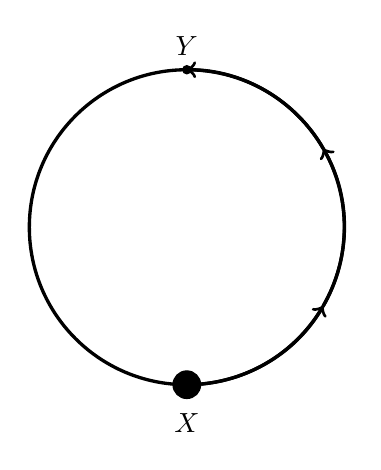
\begin{tikzpicture}
        \draw[very thick] (0,0) circle (2cm);
        %% Arrows
        \draw[very thick,->] (270:2) arc (270:330:2);
        \draw[very thick,->] (330:2) arc (-30:30:2);
        \draw[very thick,->] (30:2) arc (30:90:2);
        \draw[fill] (0,-2) circle (5pt) node[yshift=-7pt,anchor=north] {$X$};
        \draw[fill] (0,+2) circle (1.5pt) node[yshift=1.5pt,anchor=south] {$Y$};
    \end{tikzpicture}
    \end{center}
    The work done by the man is about:
    \begin{multicols}{3}
    \begin{choices}
         \wrongchoice{\SI{1}{\joule}}
         \wrongchoice{\SI{2}{\joule}}
       \correctchoice{\SI{4}{\joule}}
         \wrongchoice{\SI{6}{\joule}}
         \wrongchoice{\SI{12}{\joule}}
    \end{choices}
    \end{multicols}
\end{question}
}

\element{halliday-mc}{
\begin{question}{halliday-ch07-q62}
    A woman lifts a barbell \SI{2.0}{\meter} in \SI{5.0}{\second}.
    If she lifts it the same distance in \SI{10}{\second},
        the work done by her is:
    \begin{multicols}{2}
    \begin{choices}
        \wrongchoice{four times as great}
        \wrongchoice{two times as great}
      \correctchoice{the same}
        \wrongchoice{half as great}
        \wrongchoice{one-fourth as great}
    \end{choices}
    \end{multicols}
\end{question}
}

\element{halliday-mc}{
\begin{question}{halliday-ch07-q63}
    An escalator is used to move 20 people (\SI{60}{\kilo\gram} each)
        per minute from the first floor of a department store to the second floor,
        \SI{5}{\meter} above. 
    \begin{center}
    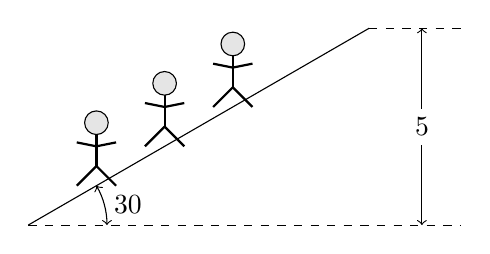
\begin{tikzpicture}
        %% Surface
        \draw (0,0) -- (30:5);
        \draw[dashed] (30:5) -- (5.5,2.5);
        \draw[dashed] (0,0) -- (5.5,0);
        \draw[<->] (5,0) -- (5,2.5) node[pos=0.5,anchor=center,fill=white] {\SI{5}{\meter}};
        %% Angle
        \draw[<->] (0:1) arc (0:30:1) node[pos=0.5,anchor=west] {\ang{30}};
        %% Man
        \foreach \x in {1,2,3} {
            \begin{scope}[anchor=south,shift={(30:\x)}]
                \draw[thick] (0,0.25) -- (0,0.75);
                %% Legs
                \draw[thick] (0,0.25) -- (-0.25,0);
                \draw[thick] (0,0.25) -- (+0.25,0);
                %% Arms
                \draw[thick] (0,0.50) -- (-0.25,0.55);
                \draw[thick] (0,0.50) -- (+0.25,0.55);
                %% Head
                \draw[fill=white!90!black] (0,0.80) circle (0.15cm);
            \end{scope}
        }
    \end{tikzpicture}
    \end{center}
    Neglecting friction, the power required is approximately:
    \begin{multicols}{2}
    \begin{choices}
        \wrongchoice{\SI{100}{\watt}}
        \wrongchoice{\SI{200}{\watt}}
      \correctchoice{\SI{1000}{\watt}}
        \wrongchoice{\SI{2000}{\watt}}
        \wrongchoice{\SI{60 000}{\watt}}
    \end{choices}
    \end{multicols}
\end{question}
}

\element{halliday-mc}{
\begin{question}{halliday-ch07-q64}
    A person holds an \SI{80}{\newton} weight \SI{2}{\meter} above the floor for \SI{30}{\second}.
    The power required to do this is:
    \begin{multicols}{2}
    \begin{choices}
        \wrongchoice{\SI{80}{\watt}}
        \wrongchoice{\SI{40}{\watt}}
        \wrongchoice{\SI{20}{\watt}}
        \wrongchoice{\SI{10}{\watt}}
      \correctchoice{none of the provided}
    \end{choices}
    \end{multicols}
\end{question}
}

\element{halliday-mc}{
\begin{question}{halliday-ch07-q65}
    A \SI{50}{\newton} force is the only force on a \SI{2}{\kilo\gram} object that starts from rest. 
    When the force has been acting for \SI{2}{\second} the rate at which it is doing work is:
    \begin{multicols}{3}
    \begin{choices}
        \wrongchoice{\SI{75}{\watt}}
        \wrongchoice{\SI{100}{\watt}}
        \wrongchoice{\SI{1000}{\watt}}
      \correctchoice{\SI{2500}{\watt}}
        \wrongchoice{\SI{5000}{\watt}}
    \end{choices}
    \end{multicols}
\end{question}
}

\element{halliday-mc}{
\begin{question}{halliday-ch07-q66}
    A \SI{50}{\newton} force is the only force a \SI{2}{\kilo\gram} crate that starts from rest. 
    At the instant the object has gone \SI{2}{\meter} the rate at which the force is doing work is:
    \begin{multicols}{3}
    \begin{choices}
        \wrongchoice{\SI{2.5}{\watt}}
        \wrongchoice{\SI{25}{\watt}}
        \wrongchoice{\SI{75}{\watt}}
        \wrongchoice{\SI{100}{\watt}}
      \correctchoice{\SI{500}{\watt}}
    \end{choices}
    \end{multicols}
\end{question}
}

\element{halliday-mc}{
\begin{question}{halliday-ch07-q67}
    A particle starts from rest and is acted on by a net force that does work at a rate that is proportional to the time $t$. 
    The speed of the particle is proportional to:
    \begin{multicols}{3}
    \begin{choices}
      \correctchoice{$\sqrt{t}$}
        \wrongchoice{$t$}
        \wrongchoice{$t^2$}
        \wrongchoice{$\dfrac{1}{\sqrt{t}}$}
        \wrongchoice{$\dfrac{1}{t}$}
    \end{choices}
    \end{multicols}
\end{question}
}


\endinput


